\documentclass[letter, 12 pt]{article}
%DIF LATEXDIFF DIFFERENCE FILE
%DIF DEL MasterThesis_old\Anteproyecto\Anteproyecto.tex   Fri May 29 01:59:04 2020
%DIF ADD MasterThesis_new\Anteproyecto\Anteproyecto.tex   Tue Jun  2 15:19:50 2020
\usepackage[utf8]{inputenc}
\usepackage[spanish]{babel}	%Español
%\usepackage[fixlanguage]{babelbib}
\usepackage{caption}		%Nombre de figuras
\usepackage{graphicx}		%Incluir figura
\usepackage{cite}			%Para guiones en citas
\usepackage{amsmath}
 
\usepackage{afterpage}		%Para dejar hojas en blanco y sin numerar
    
\usepackage{geometry}		%Tamaño de hoja y margenes
 \geometry{
 right = 3cm,
 left = 3 cm,
 top = 3 cm,
 bottom = 3cm,
 }
 
\usepackage{hyperref}		%Hipervínculos dentro del texto
\hypersetup{
    colorlinks,
    citecolor=blue,
    filecolor=black,
    linkcolor=black,
    urlcolor=blue
}

\usepackage{sectsty}

% Commands
\newcommand{\invi}{\textit{in vivo}\ }
\newcommand{\exvi}{\textit{ex vivo}\ }
%DIF PREAMBLE EXTENSION ADDED BY LATEXDIFF
%DIF UNDERLINE PREAMBLE %DIF PREAMBLE
\RequirePackage[normalem]{ulem} %DIF PREAMBLE
\RequirePackage{color}\definecolor{RED}{rgb}{1,0,0}\definecolor{BLUE}{rgb}{0,0,1} %DIF PREAMBLE
\providecommand{\DIFaddtex}[1]{{\protect\color{blue}\uwave{#1}}} %DIF PREAMBLE
\providecommand{\DIFdeltex}[1]{{\protect\color{red}\sout{#1}}}                      %DIF PREAMBLE
%DIF SAFE PREAMBLE %DIF PREAMBLE
\providecommand{\DIFaddbegin}{} %DIF PREAMBLE
\providecommand{\DIFaddend}{} %DIF PREAMBLE
\providecommand{\DIFdelbegin}{} %DIF PREAMBLE
\providecommand{\DIFdelend}{} %DIF PREAMBLE
\providecommand{\DIFmodbegin}{} %DIF PREAMBLE
\providecommand{\DIFmodend}{} %DIF PREAMBLE
%DIF FLOATSAFE PREAMBLE %DIF PREAMBLE
\providecommand{\DIFaddFL}[1]{\DIFadd{#1}} %DIF PREAMBLE
\providecommand{\DIFdelFL}[1]{\DIFdel{#1}} %DIF PREAMBLE
\providecommand{\DIFaddbeginFL}{} %DIF PREAMBLE
\providecommand{\DIFaddendFL}{} %DIF PREAMBLE
\providecommand{\DIFdelbeginFL}{} %DIF PREAMBLE
\providecommand{\DIFdelendFL}{} %DIF PREAMBLE
%DIF HYPERREF PREAMBLE %DIF PREAMBLE
\providecommand{\DIFadd}[1]{\texorpdfstring{\DIFaddtex{#1}}{#1}} %DIF PREAMBLE
\providecommand{\DIFdel}[1]{\texorpdfstring{\DIFdeltex{#1}}{}} %DIF PREAMBLE
\newcommand{\DIFscaledelfig}{0.5}
%DIF HIGHLIGHTGRAPHICS PREAMBLE %DIF PREAMBLE
\RequirePackage{settobox} %DIF PREAMBLE
\RequirePackage{letltxmacro} %DIF PREAMBLE
\newsavebox{\DIFdelgraphicsbox} %DIF PREAMBLE
\newlength{\DIFdelgraphicswidth} %DIF PREAMBLE
\newlength{\DIFdelgraphicsheight} %DIF PREAMBLE
% store original definition of \includegraphics %DIF PREAMBLE
\LetLtxMacro{\DIFOincludegraphics}{\includegraphics} %DIF PREAMBLE
\newcommand{\DIFaddincludegraphics}[2][]{{\color{blue}\fbox{\DIFOincludegraphics[#1]{#2}}}} %DIF PREAMBLE
\newcommand{\DIFdelincludegraphics}[2][]{% %DIF PREAMBLE
\sbox{\DIFdelgraphicsbox}{\DIFOincludegraphics[#1]{#2}}% %DIF PREAMBLE
\settoboxwidth{\DIFdelgraphicswidth}{\DIFdelgraphicsbox} %DIF PREAMBLE
\settoboxtotalheight{\DIFdelgraphicsheight}{\DIFdelgraphicsbox} %DIF PREAMBLE
\scalebox{\DIFscaledelfig}{% %DIF PREAMBLE
\parbox[b]{\DIFdelgraphicswidth}{\usebox{\DIFdelgraphicsbox}\\[-\baselineskip] \rule{\DIFdelgraphicswidth}{0em}}\llap{\resizebox{\DIFdelgraphicswidth}{\DIFdelgraphicsheight}{% %DIF PREAMBLE
\setlength{\unitlength}{\DIFdelgraphicswidth}% %DIF PREAMBLE
\begin{picture}(1,1)% %DIF PREAMBLE
\thicklines\linethickness{2pt} %DIF PREAMBLE
{\color[rgb]{1,0,0}\put(0,0){\framebox(1,1){}}}% %DIF PREAMBLE
{\color[rgb]{1,0,0}\put(0,0){\line( 1,1){1}}}% %DIF PREAMBLE
{\color[rgb]{1,0,0}\put(0,1){\line(1,-1){1}}}% %DIF PREAMBLE
\end{picture}% %DIF PREAMBLE
}\hspace*{3pt}}} %DIF PREAMBLE
} %DIF PREAMBLE
\LetLtxMacro{\DIFOaddbegin}{\DIFaddbegin} %DIF PREAMBLE
\LetLtxMacro{\DIFOaddend}{\DIFaddend} %DIF PREAMBLE
\LetLtxMacro{\DIFOdelbegin}{\DIFdelbegin} %DIF PREAMBLE
\LetLtxMacro{\DIFOdelend}{\DIFdelend} %DIF PREAMBLE
\DeclareRobustCommand{\DIFaddbegin}{\DIFOaddbegin \let\includegraphics\DIFaddincludegraphics} %DIF PREAMBLE
\DeclareRobustCommand{\DIFaddend}{\DIFOaddend \let\includegraphics\DIFOincludegraphics} %DIF PREAMBLE
\DeclareRobustCommand{\DIFdelbegin}{\DIFOdelbegin \let\includegraphics\DIFdelincludegraphics} %DIF PREAMBLE
\DeclareRobustCommand{\DIFdelend}{\DIFOaddend \let\includegraphics\DIFOincludegraphics} %DIF PREAMBLE
\LetLtxMacro{\DIFOaddbeginFL}{\DIFaddbeginFL} %DIF PREAMBLE
\LetLtxMacro{\DIFOaddendFL}{\DIFaddendFL} %DIF PREAMBLE
\LetLtxMacro{\DIFOdelbeginFL}{\DIFdelbeginFL} %DIF PREAMBLE
\LetLtxMacro{\DIFOdelendFL}{\DIFdelendFL} %DIF PREAMBLE
\DeclareRobustCommand{\DIFaddbeginFL}{\DIFOaddbeginFL \let\includegraphics\DIFaddincludegraphics} %DIF PREAMBLE
\DeclareRobustCommand{\DIFaddendFL}{\DIFOaddendFL \let\includegraphics\DIFOincludegraphics} %DIF PREAMBLE
\DeclareRobustCommand{\DIFdelbeginFL}{\DIFOdelbeginFL \let\includegraphics\DIFdelincludegraphics} %DIF PREAMBLE
\DeclareRobustCommand{\DIFdelendFL}{\DIFOaddendFL \let\includegraphics\DIFOincludegraphics} %DIF PREAMBLE
%DIF LISTINGS PREAMBLE %DIF PREAMBLE
\RequirePackage{listings} %DIF PREAMBLE
\RequirePackage{color} %DIF PREAMBLE
\lstdefinelanguage{DIFcode}{ %DIF PREAMBLE
%DIF DIFCODE_UNDERLINE %DIF PREAMBLE
  moredelim=[il][\color{red}\sout]{\%DIF\ <\ }, %DIF PREAMBLE
  moredelim=[il][\color{blue}\uwave]{\%DIF\ >\ } %DIF PREAMBLE
} %DIF PREAMBLE
\lstdefinestyle{DIFverbatimstyle}{ %DIF PREAMBLE
	language=DIFcode, %DIF PREAMBLE
	basicstyle=\ttfamily, %DIF PREAMBLE
	columns=fullflexible, %DIF PREAMBLE
	keepspaces=true %DIF PREAMBLE
} %DIF PREAMBLE
\lstnewenvironment{DIFverbatim}{\lstset{style=DIFverbatimstyle}}{} %DIF PREAMBLE
\lstnewenvironment{DIFverbatim*}{\lstset{style=DIFverbatimstyle,showspaces=true}}{} %DIF PREAMBLE
%DIF END PREAMBLE EXTENSION ADDED BY LATEXDIFF

\begin{document}

\setlength\parindent{0pt}
\renewcommand{\contentsname}{Contenido}	%Contenido
\renewcommand{\listtablename}{Índice de tablas}
\renewcommand{\tablename}{Tabla}	%Tabla
\renewcommand{\refname}{REFERENCIAS}

%Tamaño de la fuente en titulos
\sectionfont{\fontsize{12}{1}\selectfont\centering}
\subsectionfont{\fontsize{12}{1}\selectfont}
\thispagestyle{empty}

\begin{center}

%%%%%%%%%%%%%%%%%%%%%%%%%%%%%%%%%%%%%%%%%%%%%%%%%%%%%%%%%%%%%%%%%%%%%%%%%%%%%%%
%%				       			Portada

ÓPTICA ADAPTATIVA COMPUTACIONAL EN TOMOGRAFÍA DE COHERENCIA ÓPTICA SIN ESTABILIDAD DE FASE
\vfill

SEBASTIÁN RUIZ LOPERA
\vfill

ANTEPROYECTO: TESIS DE MAESTRÍA
\vfill

Director \\
Ph.D. RENÉ RESTREPO GÓMEZ \\
Área de instrumentación óptica espacial \\
Instituto Nacional de Técnica Aeroespacial \\
\vspace{\baselineskip}
Co-director \\
Ph.D. NÉSTOR URIBE PATARROYO \\
Wellman center for photomedicine \\
Harvard Medical School and Massachusetts General Hospital \\
\vfill

ESCUELA DE CIENCIAS \\
DEPARTAMENTO DE CIENCIAS FÍSICAS \\
MAESTRÍA EN FÍSICA APLICADA \\ 
UNIVERSIDAD EAFIT \\
2020
\end{center}

% Blank page after cover page
\thispagestyle{empty}
\newpage

%%%%%%%%%%%%%%%%%%%%%%%%%%%%%%%%%%%%%%%%%%%%%%%%%%%%%%%%%%%%%%%%%%%%%%%%%%%%%%%
%%				       				Contenido

\leavevmode\thispagestyle{empty}\newpage
\addtocounter{page}{-1}%
\renewcommand{\contentsname}{CONTENIDO}
\tableofcontents
\newpage
\setcounter{page}{3}

%%%%%%%%%%%%%%%%%%%%%%%%%%%%%%%%%%%%%%%%%%%%%%%%%%%%%%%%%%%%%%%%%%%%%%%%%%%%%%%
%%				       			Introducción

\section{INTRODUCCIÓN}
%  Definiciones iniciales de OCT, menciones al campo complejo: posibilidad de procesamiento, antecedentes en el grupo en posprocesamiento en OCT, aberraciones en OCT y formas de corregirlas.

En las ciencias médicas y biológicas, la interacción luz-materia ha permitido la creación de una disciplina especializada llamada \textit{óptica biomédica} o \textit{biofotónica}, la cual se ha centrado principalmente en investigación básica, formación de imagen, diagnóstico, terapia y monitoreo de enfermedades y procedimientos quirúrgicos~\cite{Keiser2016_Biophotonics}. Entre las técnicas ópticas que destacan en la biofotónica, se encuentra la \textit{tomografía de coherencia óptica} (OCT, \textit{optical coherence tomography}), una técnica de imagen tridimensional no invasiva con resolución micrométrica que opera con muestras esparsivas e inhomogéneas como los tejidos biológicos~\cite{huang1991}. OCT mide la luz retro-esparcida por la muestra mediante interferometría de baja coherencia, produciendo imágenes con resolución micrométrica gracias a la baja coherencia de las fuentes empleadas. OCT ha generado gran interés en el área de investigación de la biofotónica, ya que su sensibilidad y resolución permiten obtener información útil de muestras biológicas con diferentes características, además de que su resolución de 1-15~$\mu$m y profundidad de penetración  de $\sim$2~mm llenan un vacío existente entre otras técnicas de imagen médica como ultrasonido y microscopía confocal~\cite{drexler2015}. Adicionalmente, su operación no invasiva \exvi e \textit{in vivo}, sin marcadores y sin radiación ionizante ha llevado a que OCT haya adquirido gran relevancia médica, principalmente en la oftalmología~\cite{swanson1993, Ramos_2009}, pero también en imagen intravascular~\cite{Bouma2017_Medical}, endoscopia~\cite{Zhou_2015} y dermatología~\cite{Wang_2017}. \\ 

En OCT normalmente se emplea un sistema óptico que enfoca la luz en una pequeña región de la muestra, cuyo tamaño define la resolución lateral, y este puede generar aberraciones que deterioran la calidad de las imágenes obtenidas, degradando la visualización de estructuras finas y limitando el rango axial de formación de imagen~\cite{drexler2015}. Para evitar aberraciones ópticas, es posible emplear sistemas ópticos especializados, por ejemplo, los sistemas telecéntricos y acromáticos corrigen la aberración esférica y cromática. Una de las limitantes de los sistemas ópticos, que afecta particularmente en OCT, es que solo se puede formar una imagen enfocada o \textit{nítida} de aquellos planos de la muestra que están dentro de la región conocida como profundidad de campo (DoF, \textit{Depth-of-field}) que es propia del sistema, y los planos de la muestra que están por fuera del DoF aparecen desenfocados y por ende con una menor resolución efectiva. En el caso de OCT, esto significa que ciertos planos del tomograma estarán enfocados pero otros podrían aparecer desenfocados~\cite{drexler2015}. Para evitar esto, comúnmente se emplean sistemas con un DoF extenso, de forma tal que se cubra todo el rango axial del tomograma, sin embargo, esto se logra al costo de reducir la resolución lateral dado que existe una relación inversa entre la resolución y el DoF, que se conoce como \textit{resolution--DoF trade--off}. \\

Además de las aberraciones inherentes al sistema óptico, la muestra misma puede introducir aberraciones que también degradan la calidad de las imágenes, particularmente en oftalmología~\cite{liang1994, thibos2002}. Por esto, la corrección de aberraciones y la reducción del compromiso entre la resolución y el DoF han sido de gran interés en esta área y en aplicaciones que requieren alta resolución~\cite{pircher2017}. Para corregir las aberraciones existen dos aproximaciones, óptica adaptativa basada en hardware (HAO)~\cite{Pircher2007_Combining,felberer2014} y corrección computacional de aberraciones (CAC)~\cite{yasuno2006,ralston2007}. HAO tiene la desventaja de requerir componentes adicionales que añaden complejidad al sistema, además de que no permite reducir el compromiso entre la resolución y el DoF dado que aplica una corrección global. Esto último si es posible con CAC, que opera mediante posprocesamiento de la señal compleja de OCT, y cuya mayor desventaja es la pérdida de señal de naturaleza experimental a causa de las aberraciones presentes y no puede compensarse computacionalmente~\cite{liu2017}. En este trabajo se pretende desarrollar un método de CAC que pueda ser empleado en muchos tipos de sistemas de OCT, con el objetivo de brindar una herramienta para mejorar la calidad de las imágenes mediante posprocesamiento. Este documento presenta la propuesta del trabajo, comenzando por el planteamiento del problema en la sección~\ref{sec:planteamiento} y los objetivos del proyecto en la sección~\ref{sec:objetivos}, luego se explica un breve marco teórico sobre conceptos importantes y el estado del arte de las técnicas de CAC en la sección~\ref{sec:teoria}, y se finaliza con la descripción de la metodología y el cronograma propuestos para la ejecución del proyecto, en las secciones~\ref{sec:metodología}~y~\ref{sec:cronograma}, respectivamente.

%%%%%%%%%%%%%%%%%%%%%%%%%%%%%%%%%%%%%%%%%%%%%%%%%%%%%%%%%%%%%%%%%%%%%%%%%%%%%%%
%%			    		Planteamiento del problema

\section{PLANTEAMIENTO DEL PROBLEMA} \label{sec:planteamiento}
% Centrarse ahora solo en corrección con posprocesamiento: se requiere estabilidad de fase (definirla). Cómo se ha logrado la estabilidad de fase para lograr corregir las aberraciones con posprocesamiento, configuraciones especiales, no se puede aplicar en los sistemas típicos.

CAC ha sido objeto de investigación en OCT durante su desarrollo, ya que existe cierto interés en aplicaciones donde puede jugar un papel importante en la calidad de la imagen~\cite{liu2017}. El desarrollo de los métodos ha estado altamente ligado a los desarrollos experimentales de los sistemas y sus características, permitiendo obtener información confiable de amplitud y fase, algo crucial para lograr corregir aberraciones computacionalmente. Al basarse en un modelo común, las técnicas de CAC tienen los mismos requerimientos en cuanto al tomograma que se corrige, siendo la estabilidad de fase el requerimiento que ha adquirido más relevancia dada la dificultad experimental que representa. La \textit{estabilidad de fase} consiste en que exista una relación de fase coherente entre las señales de todas las posiciones del tomograma, es decir, que exista una \textit{correlación} de la señal en todo el volumen adquirido~\cite{Shemonski2014_Stability}. La dificultad de adquirir tomogramas con fase estable radica en que existen factores que afectan la fase, introduciendo ruido que decorrelaciona la señal, lo que afecta la estabilidad de fase e imposibilita el uso de las técnicas de CAC~\cite{Shemonski2014_Stability}. Algunos de estos factores son externos al sistema, por ejemplo el movimiento de la muestra durante la adquisición de la señal~\cite{shemonskiStabilityComputedOptical2014}, y otros son inherentes al sistema~\cite{Vakoc2005_Phase}. Esto ha sido una limitante para CAC, pues sólo ha sido alcanzable en configuraciones de OCT especificas que presentan estabilidad de fase, en algunos casos al costo de introducir otras \DIFdelbegin \DIFdel{dificultados }\DIFdelend \DIFaddbegin \DIFadd{dificultades }\DIFaddend como una mayor complejidad del montaje, restringiendo su uso tanto a nivel de investigación cómo a nivel médico~\cite{Shemonski2014_Stability, liu2017}. Es por esto que existe un interés actual por posibilitar el uso de técnicas de CAC en tomogramas adquiridos con cualquier sistema de OCT. \\

%Estos son, principalmente, cumplir el criterio de muestreo de Nyquist-Shannon y contar con estabilidad de fase~\cite{Shemonski2014_Stability}. El primero se logra barriendo correctamente la muestra con el sistema de escaneo transversal, de manera que el muestreo lateral debe ser como máximo la mitad de la resolución lateral máxima~\cite{Goodman2005_Introduction}. El segundo consiste en que el tomograma debe mantener una relación coherente entre todas las medidas, lo que significa que debe existir una correlación entre las medidas en las diferentes posiciones de la muestra~\cite{Vakoc2005_Phase}. \\

%La adquisición de tomogramas con fase estable no es un asunto trivial; solo es posible en ciertos sistemas que se basan en configuraciones especificas orientadas a obtener tomogramas con fase estable, en muchas casos, al costo de aumentar la complejidad del sistema. En los sistemas comúnmente usados, existen factores que afectan la fase del tomograma e introducen ruido de fase que decorrelaciona la señal y por ende afecta la estabilidad de fase, en cuyo caso no pueden aplicarse las técnicas de CAC~\cite{Vakoc2005_Phase}. Esta limitante ha llevado a que CAC sólo haya sido posible en configuraciones de OCT especificas, restringiendo su uso tanto a nivel de investigación cómo a nivel médico~\cite{Shemonski2014_Stability, liu2017}. \\

La cantidad de información que puede extraerse de la señal de OCT ha hecho que el posprocesamiento se convertida en una herramienta importante para la generación de imágenes de calidad y la obtención de información útil en OCT, para mejorar el diagnóstico, monitoreo y estudio de enfermedades, cómo es el caso de CAC. En este sentido, el Grupo de Óptica Aplicada de la Universidad EAFIT, en colaboración con el Wellman Center for Photomedicine de Massachussets Genegal Hospital y Harvard Medical School, han establecido una línea de proyectos colaborativos en el posprocesamiento de la señal de OCT con el fin de mejorar la calidad de las imágenes y su visualización para un mejor análisis y diagnóstico, logrando resultados satisfactorios en la reducción de \textit{speckle} en las imágenes~\cite{cuartas-velez2018} que comúnmente dificulta la visualización de la imágenes, y también en el cálculo robusto de la autocorrelación de la intensidad~\cite{Uribe-Patarroyo2020_Noise}, empleada por ejemplo en angiografía~\cite{Makita2006_Optical} y flujometría~\cite{Srinivasan2012_Optical}. Paralelamente, se han realizado montajes experimentales, como la implementación de un sistema de OCT de primera generación~\cite{Cuartas-Velez2019_Labmade} y el diseño e implementación de un espectrómetro lineal en el número de onda orientado a desarrollar un sistema de OCT de segunda generación~\cite{Ruiz-lopera2018_diseno, Ruiz-lopera2018_Design}. Adicionalmente, se desarrolló un algoritmo numérico de estabilización de fase que por su naturaleza iterativa requiere largos tiempos de computo~\cite{cuartas-velez2017}, sin embargo, a partir de esa exploración de nociones de estabilidad de fase y las herramientas desarrolladas se plantea esta nueva propuesta. \\

Dadas las limitaciones actuales de estabilidad de fase de los sistemas de OCT comunes, la propuesta para la tesis de maestría consiste en desarrollar y evaluar experimentalmente un método de posprocesamiento para corrección de aberraciones ópticas en tomogramas de fase inestable, sin requerir modificaciones experimentales en los sistemas\DIFdelbegin \DIFdel{, ampliando así }\DIFdelend \DIFaddbegin \DIFadd{. Esto permitirá ampliar }\DIFaddend la aplicabilidad de las técnicas de CAC para la mejora de la calidad de las imágenes\DIFdelbegin \DIFdel{de casi cualquier sistema }\DIFdelend \DIFaddbegin \DIFadd{, }\DIFaddend a través de la corrección de aberraciones \DIFaddbegin \DIFadd{en sistemas sin estabilidad de fase en los que no es posible el uso de las técnicas de CAC actuales, particularmente sistemas de escaneo puntual basados en fuente de barrido, una configuración experimental de OCT ampliamente usada en sistemas médicos y de investigación}\DIFaddend .
%%%%%%%%%%%%%%%%%%%%%%%%%%%%%%%%%%%%%%%%%%%%%%%%%%%%%%%%%%%%%%%%%%%%%%%%%%%%%%%
%%				       			 Objetivos

\section{OBJETIVOS} \label{sec:objetivos}

%%%%%%%%%%%%%%%%%%%%%%%%%%%%%   Objetivo general   %%%%%%%%%%%%%%%%%%%%%%%%%%%%

\subsection{Objetivo general}

Corregir aberraciones ópticas en tomografía de coherencia óptica sin estabilidad de fase mediante técnicas de posprocesamiento.

%%%%%%%%%%%%%%%%%%%%%%%%%%   Objetivos específicos   %%%%%%%%%%%%%%%%%%%%%%%%%%

\subsection{Objetivos específicos}

\begin{itemize}

    \item Establecer el estado del arte de la corrección computacional de aberraciones ópticas en tomografía de coherencia óptica.

    \item Identificar las fuentes de inestabilidades de fase y los métodos de estabilización de tomogramas adquiridos mediante tomografía de coherencia óptica.

    \item Desarrollar un método de posprocesamiento que permita estabilizar la fase y corregir las aberraciones en tomogramas adquiridos sin estabilidad de fase.

    \item Evaluar el desempeño del método con datos experimentales \invi y \exvi con sistemas típicos con inestabilidades de fase.

    \item Identificar y analizar las posibles limitaciones del método.

\end{itemize}


%%%%%%%%%%%%%%%%%%%%%%%%%%%%%%%%%%%%%%%%%%%%%%%%%%%%%%%%%%%%%%%%%%%%%%%%%%%%%%%
%%				        		Marco teórico

\section{MARCO TEÓRICO} \label{sec:teoria}
% Introducir OCT, explicar la idea básica. Mostrar esquema genérico.

En medicina, las técnicas de tomografía funcionan mediante la medición del retro-esparcimiento de ondas que se hacen incidir sobre la muestra, logrando así obtener información del interior de los tejidos biológicos~\cite{guy2005}. Por ejemplo, en el caso del ultrasonido se emplean ondas sonoras y se mide el eco, compuesto por la magnitud y el tiempo de retraso de las ondas que son reflejadas por la muestra~\cite{szabo2004}. Bajo esta idea, surge la tomografía de coherencia óptica donde se emplea luz en lugar de sonido, y se mide el ``eco" de la luz reflejada en términos de diferencias de longitudes de camino óptico mediante interferometría de baja coherencia~\cite{huang1991}. Para esto se emplea una fuente de luz de espectro ancho (50--200~nm) que es dividida en dos caminos, uno para el espejo de referencia y otro para la muestra de interés, tal como en un interferómetro de Michelson o de Mach-Zenhder~\cite{drexler2015}. La interferencia solo se produce cuando la diferencia de camino óptico entre el haz reflejado por la muestra y el haz de referencia se encuentre dentro de la longitud de coherencia de la fuente, determinada por su ancho espectral~\cite{huang1991}. Esto significa que la resolución con la que se puede diferenciar la información de la muestra en profundidad equivale a la longitud de coherencia de la fuente. Al tratarse de una técnica de reflectometría, el contraste de la señal de OCT se basa en cambios en el índice de refracción de la muestra~\cite{drexler2015}. \\

Los avances tecnológicos en OCT han permitido la obtención de tomogramas con condiciones suficientes para llevar a cabo técnicas de posprocesamiento que mejoran la calidad de las imágenes, técnicas que no eran posibles o estaban limitadas en los primeros sistemas de OCT, entre las que se encuentra la corrección digital de aberraciones. Es por esto que para entender el funcionamiento y el avance de CAC, es importante describir el funcionamiento de las configuraciones básicas de OCT. A continuación, se describen las configuraciones más comunes de OCT y su comportamiento frente a la estabilidad de fase, que establece una gran limitación para CAC, y luego se describen las técnicas existentes.

	\subsection{Configuraciones de OCT}
% Bajo la idea básica, explicar los tres tipos de configuraciones. Hacer mención a sistemas de campo completo y sus ventajas y desventajas.

En OCT hay un desacople entre el escaneo axial, definido en dirección de la propagación de la luz, y el escaneo transversal o lateral, que se realiza en el plano perpendicular al eje axial~\cite{drexler2015}. El escaneo axial depende de la componente interferométrica de OCT, y se define por cómo se produzca y se capture la interferencia según sean la fuente de iluminación, el espejo de referencia y el detector, lo que da pie a dos generaciones de sistemas. En la primera generación, OCT en el dominio del tiempo (TD--OCT, \textit{Time--Domain} OCT), el escaneo en profundidad de la muestra se realiza desplazando axialmente el espejo de referencia y capturando en cada posición la intensidad de la interferencia con un fotodetector, obteniendo una señal de intensidad en función de la profundidad conocida como \textit{A--line}~\cite{huang1991}. Esta configuración opera a una baja velocidad de escaneo ($\sim<$2~kHz) por limitaciones mecánicas del sistema de actuación para desplazar el espejo de referencia. Además, presenta una baja sensibilidad y limitada profundidad máxima de detección por el hecho de que la intensidad de cada punto se captura en momentos diferentes, por lo que cualquier cambio en la muestra o en el sistema puede afectar la señal. Por esta razón, en TD--OCT se requieren en general muestras estáticas, fuentes de iluminación estables y sistemas de actuación del espejo precisos, lo que limita las aplicaciones~\cite{drexler2015}. \\

La segunda generación de OCT opera en el dominio de Fourier (FD--OCT, \textit{Fourier--Domain} OCT) y consiste en mantener el espejo de referencia estático y realizar el escaneo axial de la muestra midiendo la señal de interferencia en el dominio espectral en lugar de medirla en el dominio temporal, siendo estos dominios conjugados que se relacionan mediante la transformada de Fourier~\cite{Fercher1995_Measurement}. Esta configuración presenta la ventaja de que el espectro medido contiene información de todas las profundidades, lo que mejora la sensibilidad del sistema ya que se mide la interferencia de todas las profundidades al mismo tiempo~\cite{Leitgeb2003_Performance}, además que opera a mayor velocidad comparada con TD--OCT, ventajas que extendieron el alcance de OCT y potenciaron su importancia en el diagnostico médico, al permitir, por ejemplo, obtener imágenes \invi de la retina~\cite{Nassif2004_Vivo}. La estrategia para capturar el espectro de la interferencia en FD--OCT da pie a dos tipos de configuraciones. En OCT del dominio espectral (SD--OCT, \textit{Spectral--Domain} OCT), se emplea un espectrómetro como detector~\cite{Fercher1995_Measurement}, mientras que en OCT con \DIFdelbegin \DIFdel{fuerte }\DIFdelend \DIFaddbegin \DIFadd{fuente }\DIFaddend de barrido (SS--OCT, \textit{wavelength--Swept--Source} OCT), se emplea un fotodetector como en TD--OCT y se reemplaza la fuente de iluminación que tiene un espectro ancho fijo por una fuente que emite luz con un espectro angosto pero cuya longitud de onda central instantánea se barre dentro de un ancho espectral grande~\cite{Chinn1997_Optical}. El uso de una fuente con espectro angosto lleva a que este esquema se denote como formación de imagen en el dominio de frecuencia óptica (OFDI, Optical Frequency Domain Imaging)~\cite{Yun2003_High}. Esta configuración presenta ventajas como una mayor tasa de adquisición, entre 100--400kHz~\cite{Oh2010_400}, alta sensibilidad y amplio rango de escaneo axial~\cite{Choma2003_Sensitivity}. \\

La diferenciación anterior de las configuraciones de OCT se centra en la forma cómo se produce y captura la interferencia con la que se realiza el escaneo axial de la muestra. En todas estas, típicamente se emplea un escaneo confocal con un sistema óptico que enfoca la luz en la muestra, de manera que se analiza sólo la zona iluminada según sea el tamaño del haz enfocado, y el escaneo transversal se realiza mediante espejos galvanómetros que desplazan el haz en el plano transversal, cambiando así el punto de enfoque, lo que se conoce como OCT de escaneo puntual. Al barrer el haz en una dirección y capturar un \textit{A--line} en cada punto del barrido, se obtiene una imagen de la sección transversal de la muestra conocida como \textit{B--scan}. Luego, al barrer el haz en una dirección ortogonal a la anterior y capturar una \textit{B--scan} en cada punto del barrido se obtiene un volumen o tomograma de la muestra. Sin embargo, existe otra configuración en la que se ilumina toda el área de la muestra a la vez, es decir, se emplea un haz expandido en lugar de un haz enfocado, y se utiliza un sistema óptico para formar imagen de la muestra en un detector CCD bidimensional, que permite capturar la interferencia de todos los puntos transversales en paralelo, en lugar de capturar un punto a la vez~\cite{Dubois2006_Full}. La señal capturada corresponde a una sección transversal de la muestra para un plano axial fijo llamada \textit{en--face}. Esta configuración se conoce como OCT de campo completo (FF--OCT, \textit{Full--Field OCT})~\cite{Dubois2006_Full} y puede emplearse en TD--OCT~\cite{Dubois2004_Ultrahigh-resolution} y en SS--OCT~\cite{Fergusson2010_vitro}, reemplazando el detector monopixel por un detector bidimensional. Sin embargo, en el caso de SD--OCT, se puede llegar máximo a un escaneo lineal en paralelo (LF--OCT, \textit{Line--Field OCT})~\cite{Nakamura2007_High-speed} y no a un escaneo bidimensional en paralelo, ya que el espectrómetro empleado detecta el espectro con un detector lineal y no un monopixel, de manera que al usar una detector bidimensional sólo se aumenta una dimensión al escaneo. En la Figura~\ref{fig:OCT_schemes}, se muestra un esquema simplificado de las configuraciones de TD--OCT, SD--OCT y SS-OCT que se acaban de describir, tanto de escaneo puntual como de campo completo. \\

\begin{figure}[h]
    \centering
    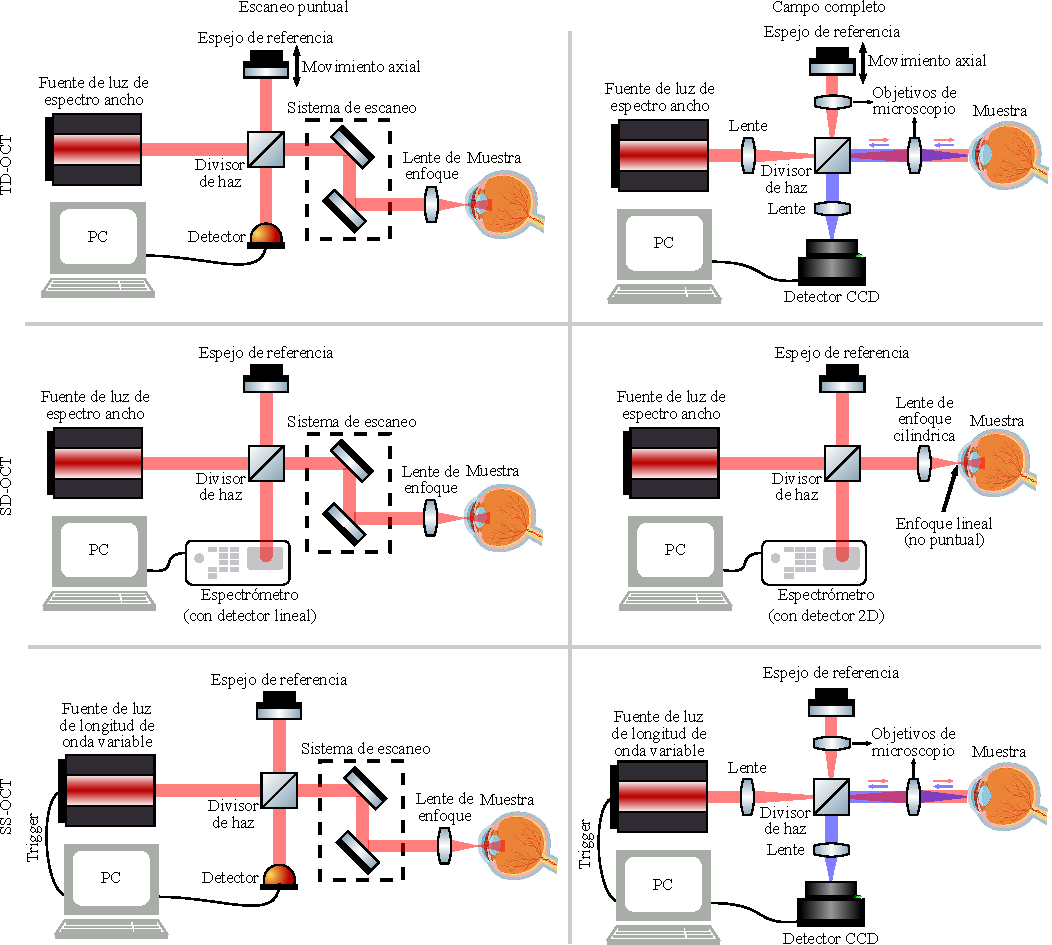
\includegraphics[width = \textwidth]{Anteproyecto/OCT_Schemes.pdf}
    \caption{Esquema simplificado de las configuraciones básicas de OCT.}
    \label{fig:OCT_schemes}
\end{figure}

El uso de sistemas de campo completo ha sido importante para el desarrollo de las técnicas de CAC como se detallará más adelante, aunque en general no son muy usados en OCT porque presentan desventajas frente a los sistemas de escaneo puntual, como una mayor complejidad experimental y mayor susceptibilidad a capturar fotones esparcidos múltiples veces.
		\subsubsection{Estabilidad de fase}
% Definir la estabilidad de fase, tiempo de interrogación, y cómo es en cada sistemas experimental.

Capturar volúmenes con fase estable ha sido un reto experimental en el campo de OCT. En general, se logra estabilidad de fase entre medidas realizadas dentro del \textit{tiempo de interrogación}, que es el tiempo durante el cual se mide la señal de un mismo punto de la muestra, aunque con sistemas de alta velocidad es posible aumentar la estabilidad de fase a varios ciclos del tiempo de interrogación~\cite{Shemonski2014_Stability}. Es por esto que los sistemas de campo completo han sido muy utilizados para CAC, ya que la adquisición en paralelo de varias posiciones laterales aumenta el tiempo de interrogación y por ende la estabilidad de fase, en comparación a sistemas de escaneo puntual~\cite{South2015_Computed}. En el caso de SD-OCT de escaneo puntual, como el espectrómetro captura la señal para todos los números de onda al mismo tiempo, el tiempo de interrogación es el tiempo de adquisición de una \textit{A--line}, por lo que existe estabilidad de fase dentro de la misma \textit{A--line} pero no entre ellas. Para lograr aplicar CAC en sistemas SD-OCT, ha sido necesario emplear espectrómetros de alta velocidad y sensibilidad, para alcanzar frecuencias de escaneo altas que permitan asumir estabilidad de fase dentro de \textit{B--scans}. Para lograr estabilidad de fase entre \textit{B--scans}, ha sido necesario emplear LF-SD-OCT con detectores CCD de alta velocidad, donde se captura una \textit{B--scan} a la vez en lugar de sólo una \textit{A--line}, lo que lleva a estabilidad de fase volumétrica~\cite{Ginner2018_Holographic}. \\

En el caso de SS-OCT, la alta velocidad de barrido de las fuentes lleva a que el tiempo de interrogación corresponda al tiempo de medida de una \textit{A--line}. De hecho, la velocidad de estos sistemas es tan alta, que en principio es posible alcanzar estabilidad de fase volumétrica con sistemas de escaneo puntual. Para esto, es necesario que exista una sincronización apropiada entre el sistema de adquisición y la fuente de barrido, de manera que en cada instante se conozca con certeza la longitud de onda que está emitiendo la fuente~\cite{Vakoc2005_Phase}. Sin embargo, en los sistemas de SS--OCT es común que exista un \textit{jitter} o tiempo de retardo en el sistema de adquisición respecto a la fuente, debido a la falta de precisión en sistemas de adquisición de alta velocidad, que produce una incertidumbre al inicio del ciclo de barrido de la fuente en relación al inicio del ciclo de adquisición. Esto produce una inestabilidad de fase conocida como \textit{phase-jitter} que restringe la estabilidad de fase a sólo dentro de \textit{A-lines}~\cite{Vakoc2005_Phase}. Es por esto que se ha demostrado el funcionamiento de CAC en SS--OCT de campo completo, donde la adquisición en paralelo elimina la presencia de \textit{phase-jitter}~\cite{kumar2013, hillmann2016}, pero aún sigue abierta su aplicación en SS--OCT de escaneo puntual, que es una de las configuraciones mas usadas en OCT y de mayor interés de desarrollo experimental y médico.

	\subsection{Aberraciones en OCT}
% Definir aberraciones, y las fuentes de aberraciones en OCT. centrarse en escaneo confocal: compromiso entre resolución lateral y profundidad de campo.

OCT es susceptible a aberraciones ópticas que pueden ser introducidas por el sistema óptico o por la muestra misma, las cuales reducen la calidad de la imagen y la capacidad de diferenciar estructuras finas. Esto ocurre de manera equivalente tanto en sistema de escaneo puntual como en sistemas de campo completo, por lo que en adelante se asumen sistemas del primero tipo. En relación al sistema óptico, la mayor limitante es que los planos por fuera de la profundidad de campo (DoF, \textit{Depth-of-Field}) se encuentran desenfocados como efecto intrínseco al sistema óptico de enfoque, por lo que la resolución lateral nominal, definida por la apertura numérica (NA) del sistema de enfoque, sólo es alcanzable dentro del DoF y se deteriora por fuera de este, evidenciándose como un emborronamiento en el tomograma capturado~\cite{drexler2015}. Existen otras fuentes de aberraciones, asociadas a la desalineación del sistema o inherentes al sistema óptico o a la muestra, como ocurre en oftalmología debido a la córnea y el cristalino~\cite{liang1994, thibos2002}. \\

Cómo se dijo anteriormente, para corregir las aberraciones, existen dos aproximaciones, óptica adaptativa basada en hardware (HAO)~\cite{pircher2017} y corrección computacional de aberraciones (CAC)~\cite{liu2017}. En HAO se modifica el sistema óptico añadiendo componentes adicionales para determinar el frente de onda aberrado, y componentes para compensar las aberraciones medidas introduciendo cambios en el frente de onda~\cite{zawadzki2011}. Una gran limitación de HAO es el hecho de que se aplica una corrección global, por lo que no permite extender el DoF ya que esto requiere una corrección específica en cada plano~\cite{pircher2017}. Por esto, y dada la complejidad y costo del montaje, HAO generalmente se emplea en oftalmología, en formación de imagen del segmento posterior del ojo, dado que las aberraciones que introduce el ojo del paciente pueden llegar a afectar considerablemente las imágenes, además de que varían entre pacientes por lo que se requiere una corrección \emph{in situ}~\cite{zawadzki2011,felberer2014}. Por otra parte, CAC se basa en posprocesamiento de la señal compleja de OCT para compensar computacionalmente las aberraciones aplicando filtros de fase apropiados, que se puede determinar de múltiples formas~\cite{liu2017, adie2012, kumar2014}, y que permiten compensar el compromiso entre resolución y DoF. \\

Inicialmente, CAC se demostró con muestras de prueba como \textit{phantoms} y muestras vegetales. Mas adelante, se aplicó exitosamente \exvi en tejido de ratón pulmonar~\cite{adie2012}, adiposo~\cite{pande2016} y cerebral~\cite{south2019}, \invi en piel humana~\cite{liu2014} y en la retina, alcanzando la visualización de células fotorreceptoras~\cite{hillmann2016,pande2016}, aplicación en la que han tomado relevancia HAO y CAC, ya que las células fotorreceptoras son útiles para el diagnóstico de varias enfermedades como la degeneración macular~\cite{liu2017}.

	\subsection{Técnicas de corrección computacional de aberraciones}
% Describir a grandes rasgos las técnicas de corrección computacional de aberraciones.

	\subsubsection{Modelo general de la señal de OCT}
% Presentar el modelo resumido de la señal compleja obtenida en OCT, desde un punto de vista de propagación de la luz y no desde un punto de vista interferometrico como en las tesis pasadas.

Aunque existen varias técnicas de CAC, el modelo que emplean es común a todas y se basa en el esquema de adquisición de OCT, entendido como un modelo de esparcimiento inverso donde, de manera resumida, la señal adquirida en el dominio espectral $s(x,y;k)$, para cada posición transversal $(x,y)$ y un número de onda $k$, se modela como la convolución ($\ast$) entre la función respuesta al impulso o PSF del sistema $h(x, y; k)$ y el potencial de esparcimiento de la muestra $\eta(x,y;q_z)$ cómo~\cite{kumar2015}
    \begin{equation}\label{eq.ConvOCT}
s(x,y;k) = h(x,y;k) * \eta(x,y;q_z),
    \end{equation}
con $q_z=-2\sqrt{k^2 - (q_x/2)^2 - (q_y/2)^2}$. Computacionalmente se puede revertir el efecto de $h(x,y;k)$, que actúa como un filtro frecuencial complejo, para obtener $\eta(x,y;q_z)$ a partir de $s(x,y;k)$ mediante deconvolución, que puede realizarse con transformadas de Fourier $\text{FT}\{\cdot\}$~\cite{kumar2015}. Para lograr una mejora significativa en la calidad de la imagen al realizar la deconvolución, la función $h(x,y;k)$ debe representar apropiadamente las aberraciones que afectan el tomograma. Las diferentes técnicas de CAC en OCT difieren en la manera de determinar el filtro de deconvolución. Las primeras implementaciones en CAC consistieron en aplicar un filtro únicamente de amplitud a la intensidad de la señal de TD-OCT~\cite{Ralston2005_Gaussian}, generando resultados bastantes limitados por no incluir información de fase que es crucial para corregir aberraciones. Si la fase del tomograma es estable, es posible usar las técnicas basadas en el campo completo que se presentan a continuación.

\subsubsection{Re-enfoque digital}

En principio, puede considerarse que FD-OCT realiza tomografía digital holográfica sintetizada con varias longitudes de onda, por lo que la señal de OCT en un plano $z$ puede entenderse con el \textit{forward model} (FM) al igual que en holografía~\cite{Yu2007_Digital}
    \begin{equation}\label{eq.refocusing}
S(q_x, q_y; z) = \exp[-iz(q_x^2 + q_y^2)/4k_c] \ast \eta(q_x, q_y; z),
    \end{equation}
que resulta de realizar la aproximación paraxial $q_z$ en la Eq.~\eqref{eq.ConvOCT}, y que consiste en la ecuación de difracción escalar, donde el término de fase cuadrático representa desenfoque intrínseco a la propagación de la luz desde la lente de enfoque hasta la muestra~\cite{yasuno2006}. El re-enfoque digital consiste en aplicar a cada imagen transversal o \textit{en--face} el término de fase inverso correspondiente para cancelar el factor de fase cuadrático de la Eq.~\eqref{eq.refocusing}. Esta implementación emplea un filtro únicamente de fase y corrige el efecto del desenfoque por fuera del DoF, lo que resulta en una extensión sintética del DoF. Sin embargo, para un correcto funcionamiento requiere conocimiento preciso de los parámetros del término de fase, como las distancias de propagación, además, de que solo opera bien en sistemas con NA baja ($\sim$0.1), que son las usadas típicamente en OCT.

\subsubsection{Microscopia interferométrica de apertura sintética}

Cuando se tienen NA grandes ($>$0.1), es necesario considerar que la región iso-planática del frente de onda no es un plano sino una superficie con cierta curvatura, generando un desenfoque tanto lateral como axial. Para corregir este efecto se debe emplear la Eq.~\eqref{eq.ConvOCT} con el término $q_z$ sin aproximación. En este caso, dicha corrección no se realiza independientemente a cada \textit{en--face} como en el caso anterior, sino que se aplica directamente a todo el volumen capturado $s(x,y;k)$. Actualmente, se ha deducido una manera directa de aplicar esta corrección, conocida como Microscopía Interferométrica de Apertura Sintética (ISAM, \textit{Interferometric Synthetic Aperture Microscopy}) donde se corrige la señal de OCT en el dominio frecuencial, para luego obtener un potencial de esparcimiento de la muestra aproximado $\tilde{\eta}(x,y,z)$ mediante una transformada inversa de Fourier $\text{FT}^{-1}\{\cdot\}$ tridimensional~\cite{ralston2007},
    \begin{equation}
\tilde{\eta}(x,y,z) = \text{FT}^{-1}\bigg\{s(q_x, q_y; k)\bigg|_{k = \frac{1}{2}\sqrt{q_x^2+q_y^2+q_z^2}}\bigg\},
    \end{equation}
lo que consiste básicamente en un re-muestreo de $k$ a $q_z$. Esta técnica, propuesta por Ralston \textit{et. al.}~\cite{ralston2007}, ha sido empleada por muchos grupos de investigación en varias configuraciones, ya que tiene una implementación relativamente simple y permite obtener imágenes de alta resolución tanto axial como lateral en un DoF extendido~\cite{Chen2010_Approximate, Chen2010_Sdoct}.

\subsubsection{Óptica adaptativa digital}

Las dos técnicas descritas anteriormente se basan en definir el filtro frecuencial para corregir el tomograma capturado, considerando únicamente la curvatura del frente de onda, que resulta en un emborronamiento que cambia en cada plano según su distancia al plano focal. Sin embargo, el tomograma capturado puede estar afectado por otros tipos de aberraciones de mayor orden, intrínsecas a la muestras, por ejemplo, astigmatismo en el ojo de un paciente~\cite{thibos2002}, o al sistema óptico, como el astigmatismo producido por la sonda empleada en OCT basada en catéter~\cite{wang2012, xi2009a}. \\

En estos casos, es necesario definir un filtro $h(x,y;k)$ más elaborado para lograr representar y corregir todas las aberraciones que afecten al tomograma, lo que se logra con óptica adaptativa computacional (CAO)~\cite{adie2012}. En esta técnica, se representa el filtro en términos de los polinomios de Zernike $Z_j$ usando una suma ponderada $\sum_j\alpha_jZ_j$, cuyos pesos $\alpha_j$ se determinan para cada \textit{en-face} y se aplican mediante deconvolución de la Eq.\eqref{eq.ConvOCT}. En CAO existen dos estrategias para determinar los pesos para producir el filtro de fase apropiada, CAO basada en optimización~\cite{adie2012, pande2016, hillmann2016} y CAO de correlación de sub-aperturas~\cite{kumar2013}. En la primera, se emplea una métrica de calidad de imagen para encontrar los pesos $\alpha_j$ que maximicen dicha métrica~\cite{adie2012}. En la segunda, se determina el frente de onda de corrección directamente en el tomograma adquirido, que luego se descomponen en los polinomios de Zernike para encontrar los pesos $\alpha_j$~\cite{kumar2013}. La determinación del frente de onda se logra dividiendo el plano de Fourier de cada \textit{en--face} en sub-aperturas y calculando la pendiente local relativa entre estas, similar al funcionamiento de un sensor Shart-Hartmann. La posibilidad de CAO de corregir aberraciones además de desenfoque, han llevado a su uso en áreas donde se alcanzan resultados comparables con HAO, como en imagen de la retina~\cite{hillmann2016, Ginner2017_Noniterative}, con la ventaja de que CAO logra exterder el DoF en contraste con HAO. Además, CAO puede complementarse con ISAM para lograr incluso mejores resultados en sistemas de alta resolución, al combinar la extensión de DoF de ISAM con la corrección de aberraciones de CAO.

%%%%%%%%%%%%%%%%%%%%%%%%%%%%%%%%%%%%%%%%%%%%%%%%%%%%%%%%%%%%%%%%%%%%%%%%%%%%%%%
%%				       			Metodología

\section{METODOLOGÍA} \label{sec:metodología}
Para el desarrollo del trabajo se proponen cinco etapas metodológicas: \textit{i.}~búsqueda bibliográfica y estudio teórico de conceptos fundamentales dentro del contexto del trabajo, \textit{ii.}~desarrollo e implementación del método para resolver el problema planteado, \textit{iii.}~evaluación experimental del método desarrollado con datos obtenidos con sistemas típicos, \textit{iv.}~análisis del método y de los resultados con el fin de determinar las limitaciones y el alcance del mismo, \textit{v.}~documentación y publicación de los resultados.

	\subsection{Revisión bibliográfica y estudio teórico}
La revisión del estado del arte establece el punto de partida para desarrollar el método que permitirá resolver el problema planteado. En esta etapa, se plantea la apropiación de conceptos importantes, para luego identificar y estudiar las técnicas computacionales existentes para corrección de aberraciones ópticas. Adicionalmente, se estudiarán las configuraciones experimentales de los sistemas para identificar las fuentes de inestabilidades de fase, así como métodos de estabilización existentes. Aunque esta etapa es constante a lo largo del trabajo, se concentra en el inicio del mismo, por tanto, en este momento se encuentra desarrollada en un 80\%. %, tanto la identificación y selección de bibliografía como el estudio de la misma. Cómo fuentes bibliográficas se tienen las revistas de impacto en el área de la óptica que se concentran en editoriales de organizaciones como OSA, SPIE e IEEE, y como bases de datos se cuenta con las herramientas Scopus y ScienceDirect.

	\subsection{Desarrollo e implementación}
A partir del estudio bibliográfico, y con el entendimiento del funcionamiento de las técnicas de CAC y estabilización de fase en OCT, en esta etapa se procederá a desarrollar e implementar el método para resolver el problema planteado. Para esto, se seleccionará alguna o varias técnicas de CAC, teniendo como referencia sus ventajas y desventajas. Igualmente, se implementará un algoritmo de estabilización de fase completamente computacional, que no dependa directamente de componentes físicas en el sistema. La programación de los algoritmos se realizará en MATLAB empleando una estación de computo Dell Precision Tower 3630 Intel Core i7-9700 @ 3.0~Ghz con memoria de 64~GB, usando datos de prueba ya disponibles que consisten en tomogramas de OCT simulados que presentan desenfoque. Al tratarse de datos simulados, estos son estables en fase, así que se introducirá una inestabilidad de fase conocida y se evaluará el resultado del algoritmo de estabilización de fase teniendo como referencia la fase original. Con estos datos se realizarán las pruebas conceptuales para plantear y desarrollar el método general integrando y complementando los algoritmos programados.

	\subsection{Evaluación experimental}
Se realizarán pruebas de concepto enfocadas a una validación y depuración del método planteado, usando tomogramas experimentales que se adquirieron con un sistema OFDI que emplea una fuente de luz basada en espejo poligonal y que presenta una alta inestabilidad de fase. Los tomogramas son de una muestra de \textit{cucumis sativus}, que presenta estructuras claras y de bajo esparcimiento múltiple, características apropiadas para validar el método. Se cuenta con dos tomogramas, uno \DIFdelbegin \DIFdel{de referencia }\DIFdelend donde se ajustó el enfoque experimentalmente, \DIFaddbegin \DIFadd{que puede asumirse como una referencia sin aberraciones significativas, }\DIFaddend y otro que se adquirió desplazando el plano focal para obtener una versión aberrada por desenfoque. Con el método propuesto se espera que el tomograma aberrado puede enfocarse computacionalmente para aproximarse al tomograma enfocado experimentalmente. En \DIFaddbegin \DIFadd{esta prueba de concepto se evaluará la corrección de desenfoque ya que es la aberración más común en los sistemas de OCT, siendo otras aberraciones ópticas como esférica y cromática corregidas usando sistemas ópticos especializados para ello. }\\

\DIFadd{En }\DIFaddend un segundo paso, se evaluará el funcionamiento del método en tomogramas de muestras con relevancia médica, donde las condiciones experimentales y la naturaleza del tejido mismo imponen dificultades para su operación en comparación con los \DIFdelbegin \DIFdel{dos }\DIFdelend casos anteriores. \DIFaddbegin \DIFadd{En este caso, los tomogramas pueden presentar desenfoque al igual que otras aberraciones debidas a las muestras, las cuales pueden ser corregibles con técnicas de CAO. }\DIFaddend Se cuenta con \DIFaddbegin \DIFadd{tomgoramas adquiridos con diferentes sistemas de OFDI; }\DIFaddend un tomograma \invi del tracto respiratorio de un cerdo empleando un catéter, \DIFdelbegin \DIFdel{con }\DIFdelend tomogramas \exvi del segmento anterior del ojo de un cerdo con diferentes planos de enfoques en la región de la cornea y del iris, y \DIFdelbegin \DIFdel{con }\DIFdelend tomogramas \invi de la piel del dorsal de la mano de una persona, donde es necesario tener en cuenta el movimiento involuntario.

    \subsection{Análisis del método y de resultados}
En el análisis de resultados se plantea una evaluación cualitativa inicial, basada en la comparación visual de los tomogramas originales y luego de aplicar el método respecto a las referencias enfocadas experimentales. Posteriormente, para una correcta evaluación del método, será necesario establecer un criterio cuantitativo de comparación \DIFdelbegin \DIFdel{, basado en }\DIFdelend \DIFaddbegin \DIFadd{usando }\DIFaddend una métrica de calidad de imagen\DIFaddbegin \DIFadd{, por ejemplo, la relación señal-ruido o las métricas de }\textit{\DIFadd{nitidez}} \DIFadd{basadas en la intensidad o en el espectro de Fourier}\DIFaddend . Luego del análisis cualitativa y cuantitativo el método, es necesario identificar los requerimientos y el alcance de este. Por un lado, se deberá determinar bajo qué condiciones opera, en decir, los requerimientos básicos, en términos de parámetros experimentales o computacionales. Así mismo, es importante establecer el alcance de este, por ejemplo, en términos de las aberraciones que pueden corregirse exitosamente y las características ópticas de las muestras o tejidos. Esto permitirá establecer diferencias entre los resultados obtenidos con una corrección computacional de aberraciones respecto a un tomograma sin aberraciones desde la adquisición, específicamente desenfoque en el caso de los tomogramas de prueba.

	\subsection{Documentación y publicación de resultados}
Las actividades de documentación y publicación de resultados incluyen la estructuración y redacción del documento final de la tesis de maestría, donde se recopila la información pertinente del trabajo, así cómo de la defensa pública requerida. Por otro lado, para la divulgación de los resultados, se espera realizar por lo menos una publicación en una revista de impacto y una presentación oral en un evento nacional o internacional reconocido para lograr una difusión y retroalimentación de los resultados. % Aunque esta etapa se concentra al final del periodo de ejecución del trabajo, espera realizarse transversalmente a lo largo de este, documentando periódicamente los avances alcanzados.

%%%%%%%%%%%%%%%%%%%%%%%%%%%%%%%%%%%%%%%%%%%%%%%%%%%%%%%%%%%%%%%%%%%%%%%%%%%%%%%
%%				       				Cronograma

\section{CRONOGRAMA} \label{sec:cronograma}

El cronograma se ha dividido en dos años, en el 2019 (Figura~\ref{fig:2019}) se realizaron dos etapas que consistieron en la exploración inicial y la revisión bibliográfica y estudio teórico, mientras que las etapas de desarrollo se constituyen en el 2020 (Figura~\ref{fig:2020}). El nivel de gris indica la intensidad de trabajo, siendo oscuro la mayor intensidad. \DIFaddbegin \DIFadd{La semana 3 de septiembre del 2020 corresponde a la entrega del documento escrito para su evaluación.}\DIFaddend \\

\DIFdelbegin %DIFDELCMD < \begin{figure}
%DIFDELCMD <     %%%
\DIFdelendFL \DIFaddbeginFL \begin{figure}[h]
    \DIFaddendFL \centering
    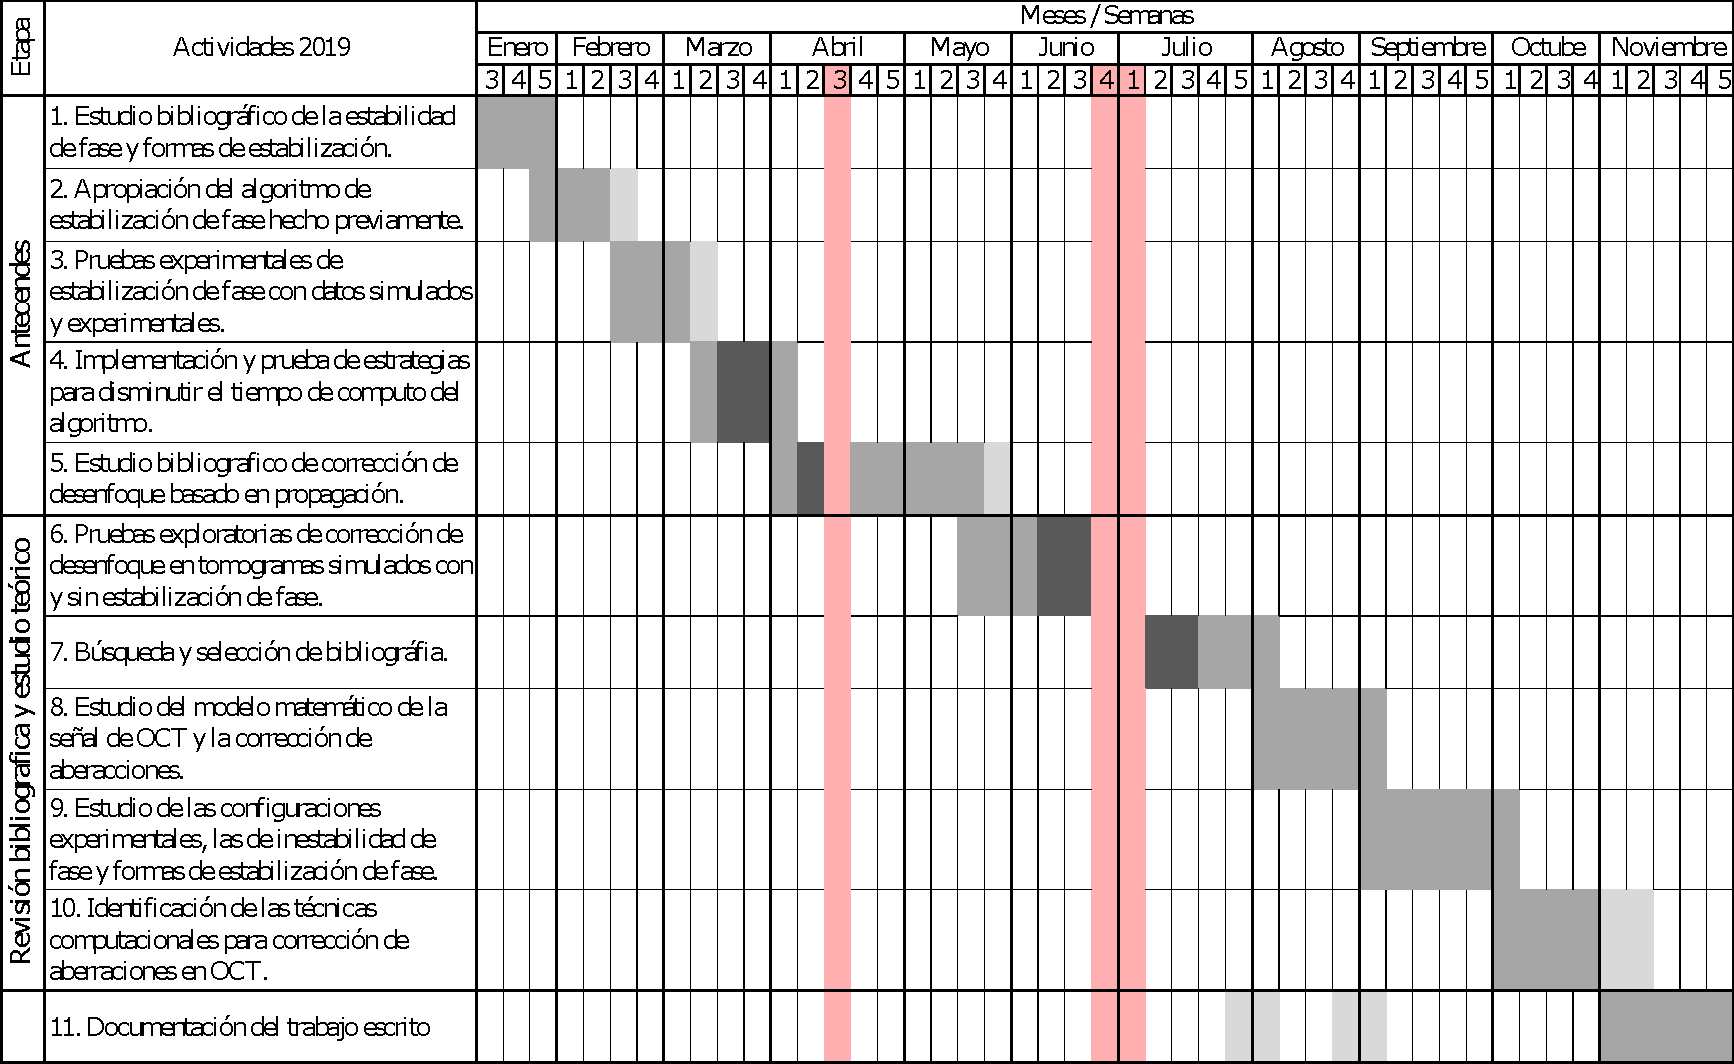
\includegraphics[width=\textwidth]{Anteproyecto/Cronograma1.pdf}
    \caption{Cronograma de actividades del 2019.}
    \label{fig:2019}
\end{figure}
\DIFdelbegin %DIFDELCMD < \begin{figure}
%DIFDELCMD <     %%%
\DIFdelendFL \DIFaddbeginFL \begin{figure}[h]
    \DIFaddendFL \centering
    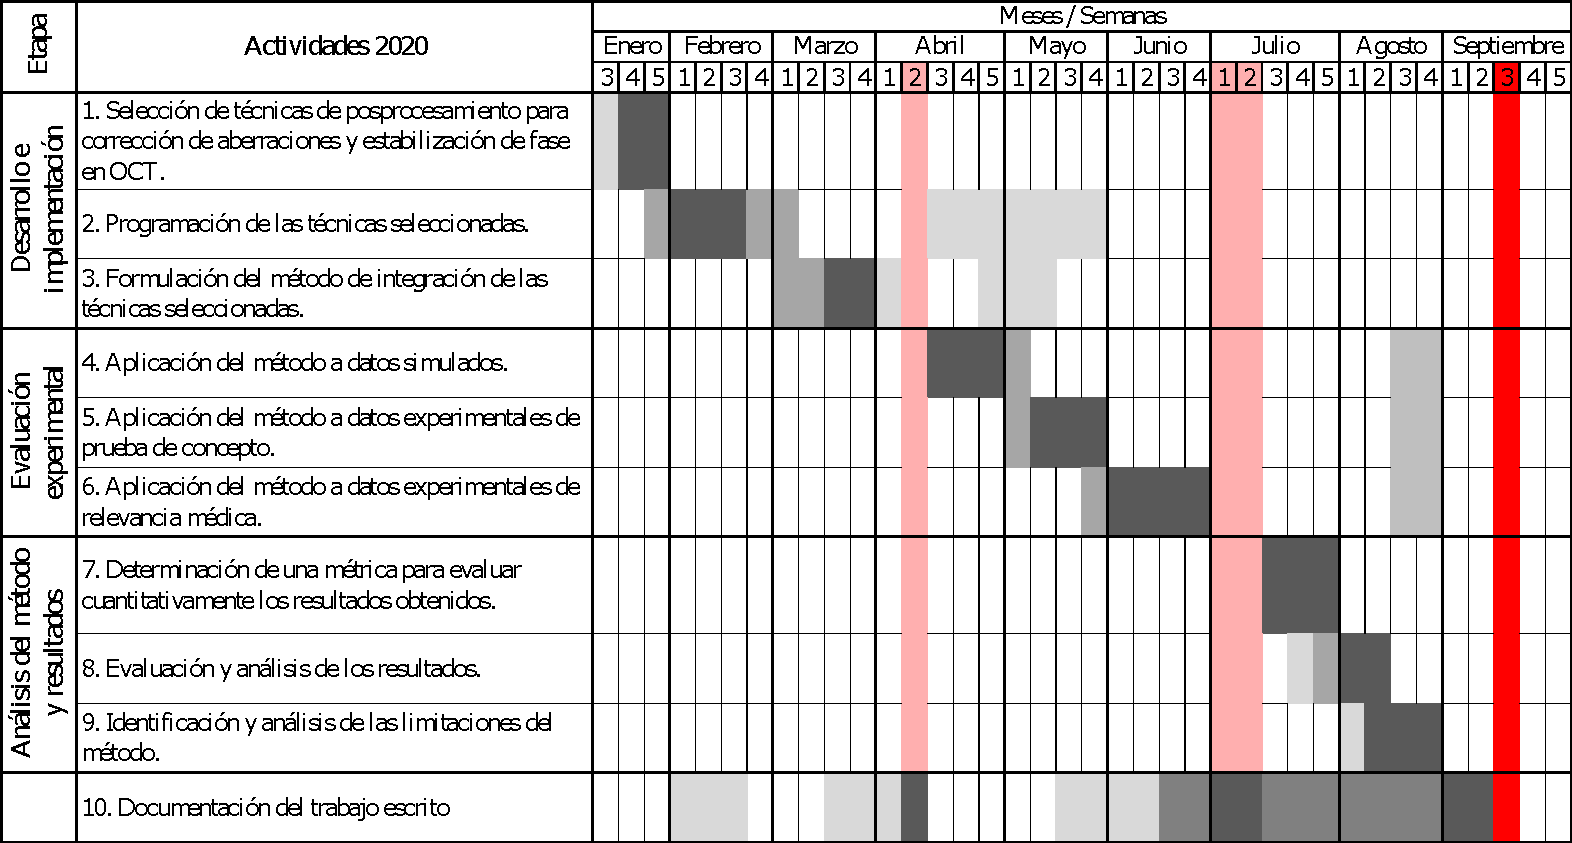
\includegraphics[width=\textwidth]{Anteproyecto/Cronograma2.pdf}
    \caption{Cronograma de actividades del 2020.}
    \label{fig:2020}
\end{figure}
%%%%%%%%%%%%%%%%%%%%%%%%%%%%%%%%%%%%%%%%%%%%%%%%%%%%%%%%%%%%%%%%%%%%%%%%%%%%%%%
%%				      				Referencias

\newpage
\addcontentsline{toc}{section}{REFERENCIAS}
%\bibliographystyle{babunsrt-fl}
\bibliographystyle{unsrt}
\bibliography{Anteproyecto/AnteproyectoBibsource.bib}

\end{document}
